% Document class, paper size, base font size
\documentclass[a4paper, 12pt]{article}

% Encoding
\usepackage[utf8]{inputenc}
\usepackage[T1]{fontenc}

% Prevent indentation of beginning of paragraphs
\setlength{\parindent}{0em}

% Space between paragraphs
\parskip 0.5em

% include PDFs
%\usepackage{pdfpages}

% Farben
\usepackage[dvipsnames]{xcolor}

% For Check-List
\usepackage{enumitem}
\usepackage{amssymb,wasysym}
\usepackage{graphicx}
\usepackage{enumerate}
\newlist{todolist}{itemize}{2}
\setlist[todolist]{label=$\square$}

% Title, authors and date
\title{Software Engineering - Analysis\\
Project: E-Scooter Rental Service}

\author{
    Kendra Birringer (1229372)\\
    Nader Cacace (1208115)\\
    Steffen Hanzlik (1207417)\\
    Marco Peluso (1228849)\\
    Svetozar Stojanovic (1262287)\\
    \\
    Frankfurt University of Applied Sciences
}
\date{February 15th, 2020}


% Begin actual document
\begin{document}

\maketitle
\newpage
\tableofcontents

\newpage
\section{Introduction}
In this project, we will take the role of founding a start-up company in the E-Scooter rental business.
For analyzing this project, our team decided to use the agile method SCRUM.

The purpose of this project is to get a clear understanding of requirements, to develop use cases and diagrams using UML to describe the planned system using a model-based software engineering approach.
Furthermore, the objective is to develop a high-level software architecture and build user interface (UI) prototypes for relevant parts of the functionality.
For our project, the artifacts consist of diagrams and documentation for describing the software functionality for outsourcing the development. The quality of these artifacts will be ensured by a proper definition of "Done".

The first step of our project is to collect additional requirements and refine these to build a list of backlog items and to estimate the time needed for producing the artifacts for each backlog item. The purpose of a backlog item is to take a requirement description, in form of a use case description, as input and build an analysis model of our software capability as result.

\section{Definition of "Done"}
The definition of "Done" (DoD) is part of the SCRUM metrics. All members of the Scrum Team must have a shared understanding of what it means when the work is complete, to ensure transparency. \cite{scrumguide}
It is a (check-)list of items which need to be validated to consider a backlog item being “Done”. DoD is defined by the development organization to make sure that the results of multiple teams can be integrated into a releasable product. \cite{thoma1}

For our project, the result needs to match the following definition of "Done":
\begin{todolist}

\item Description of the requirement in form of a Use Case
\item Categorization of requirement (functional/non-functional,\\
      client/server)
\item Business value of the corresponding functionality
\item Effort estimation for the implementation of the requirement
\item For UI related functions: UI prototype
\item UML Diagrams 

    $\bullet$ Use case diagram
    
    $\bullet$ Activity diagram
    
    $\bullet$ Class diagram
    
    $\bullet$ Sequence diagram
    
\item Detailed documentation (e.g. table) about who worked on the item and what has been done during the sprint.
\item Overall quality of the documentation meets general industry standards.
\item The results have been reviewed and accepted by another member of the team (tester). It needs to be documented who has performed the review.

\end{todolist}


%==============================================================================
\section{Backlog Items}
Backlog items are part of a product backlog. This is an ordered list of requirements which have to be done for the product.

Below we present our collected backlog items in from of a table.

\color{red}TODO: INSERT BACKLOG ITEMS LIST HERE!\color{black}


%==============================================================================
\section{Week One}
%==============================================================================
In the first week our team started to collect requirements for the E-Scooter rental service project. We discussed which requirements could fit and saved them in a Google Sheets document, to make it easy for us to collaborate on the requirements, even if we weren't in the same location. We also started to talk about the estimation, satisfactions and disatisfactions, the priority, what each requirement should do and when it would fit.
Then we thought about how an E-Scooter should work and interact with the customers.
In order to understand how the main concept of renting an E-Scooter is, some team members rented an E-Scooter from the company "Lime" to gain some first hand experience.

The task for each team member for this week was to collect more requirements for the project.
Because finding dates for further meetings turned out to be difficult, we decided to hold our meetings weekly or whenever there would occur any problems which needed to be discussed, via Discord. Discord is an "All-in-one voice and text chat [\ldots] that's free, secure, and works on both your desktop and phone."\cite{discord}

\subsection{Division of Work: Week One}
\begin{table}[h]
\centering
\setlength{\tabcolsep}{10pt}
\begin{tabular}{|c|c|c|c|c|}
\hline
K. Birringer & N. Cacace & S. Hanzlik & M. Peluso & S. Stojanovic\\
\hline
\% & \% & \% & \% & \% \\ 
\hline
\end{tabular}
\end{table}

%==============================================================================
\section{Week Two}
%==============================================================================
Since we decided to use the agile method Scrum for analyzing the E-Scooter rental service project, the team members were assigned the following roles:

\begin{itemize}
\item Scrum Master: Kendra Birringer

As Scrum Master she was responsible for the organization of the whole team: she organized and moderated the team meetings and wrote the protocols. 

Another task was to check and correct the spelling, grammar and contents of everything that was written.

\item Development Team: Nader Cacace, Steffen Hanzlik,\\
      Svetozar Stojanovic

The Development Team was responsible for modeling all neccessary UML diagrams and sketching UI prototypes.

\item Tester: Marco Peluso

The Tester mainly reviewed, documented and accepted the resulting artifacts.
\end{itemize}


In the second week the team discussed each of the collected requirements, and we decided which of them fit and which are not necessary for the software. During this discussion we gathered more requirements.

Then we started to talk about the UML diagrams and built a first use case diagram which was too big and complex and needed some adjustments. So, the task for the Development Team was to simplify the diagram and make it clearer.

Also, we built a main structure for the documentation of the project and started writing the documentation.

\newpage
\subsection{Division of Work: Week Two}

\begin{table}[h]
\centering
\setlength{\tabcolsep}{10pt}
\begin{tabular}{|c|c|c|c|c|}
\hline
K. Birringer & N. Cacace & S. Hanzlik & M. Peluso & S. Stojanovic\\
\hline
\% & \% & \% & \% & \% \\ 
\hline
\end{tabular}
\end{table}
%==============================================================================
\section{Week Three}
%===============================================================================
In week three the Development Team modified the use case diagram which was too big. They also modeled further use case diagrams which we then disussed, to find out if they needed further adjustments. At the end of this week, we finished the use case diagrams and finally added the use case documentation to each use case.

Also, after we thought about where it could be necessary, some activity and sequence diagrams were modeled.
Regarding the sequence diagrams there were some problems.
For example, the "Check-in" diagram:

We asked ourselves how to calculate the price for a ride. After some discussion we decided to let the wallet calculate the price for the ride information from the Scooter.
First, the payment also was included in this diagram, but after reconsidering, we decided that the payment also needed its own, more detailed diagram. In the end, both diagrams are very connected.

Considering the acitivity diagrams, we decided to not model a diagram for "Give feedback", because it seemed too simple.

Then we started to think about the class diagram and asked ourself which classes we needed and which relations the different classes could have to each other and started modeling the class diagram.

Furthermore, a first UI prototype was built with the sofware design tool "Axure".\cite{axure}

\newpage
\subsection{Division of Work: Week Three}

\begin{table}[h]
\centering
\setlength{\tabcolsep}{10pt}
\begin{tabular}{|c|c|c|c|c|}
\hline
K. Birringer & N. Cacace & S. Hanzlik & M. Peluso & S. Stojanovic\\
\hline
\% & \% & \% & \% & \% \\ 
\hline
\end{tabular}
\end{table}

%==============================================================================
\section{Week Four}
%===============================================================================
During week four we refined the state of the project by doing a lot of adjustments and modifications to everything we had done, so far.
We updated the requirements, checked spelling and grammar, put the requirements in a proper order and checked what was still missing.

On the basis of the backlog items list we finished all UML diagrams and UI prototypes.
After we heard the lecture, in which Prof. Dr.-Ing Peter Thoma talked about UML diagrams, we  noticed, that all our activity diagrams lacked a cancelation mode. Therefore, we had to adjust all these diagrams and add a cancelation mode to them. 

We also finished most of the documentation, so that almost only the appendices needed to be added.

The goal of our team was, to finish everything until the end of this week, so that in the following week, we would be able to fully concentrate on the presentation of the project.

\subsection{Division of Work: Week Four}

\begin{table}[h]
\centering
\setlength{\tabcolsep}{10pt}
\begin{tabular}{|c|c|c|c|c|}
\hline
K. Birringer & N. Cacace & S. Hanzlik & M. Peluso & S. Stojanovic\\
\hline
\% & \% & \% & \% & \% \\ 
\hline
\end{tabular}
\end{table}
%==============================================================================
\section{Week Five}
%===============================================================================
In week five, we checked everything again and finished everything.
We generated the report from MagicDraw and added it to the documentation.
Also, we added all protocols from the team meetings.

Then we thought about a way, how to integrate the UI prototypes. We decided to screenshot each prototype and added them as an appendix to the documentation of the project.

Once the documentation was finished, each team member proofread it again and made any necessary improvements, corrections and additions.

Then, finally we started to talk about the presentation and started to build it.

%==============================================================================
\subsection{Division of Work: Week Five}

\begin{table}[h]
\centering
\setlength{\tabcolsep}{10pt}
\begin{tabular}{|c|c|c|c|c|}
\hline
K. Birringer & N. Cacace & S. Hanzlik & M. Peluso & S. Stojanovic\\
\hline
\% & \% & \% & \% & \% \\ 
\hline
\end{tabular}
\end{table}
%==============================================================================

\newpage    
%==============================================================================
\begin{thebibliography}{}
\bibitem{scrumguide}
https://www.scrumguides.org/scrum-guide.html

\bibitem{thoma1}
Prof. Dr.-Ing Peter Thoma \emph{02-3 Software Engineering Analysis (Scrum)}
 
\bibitem{discord}
https://discordapp.com/
 
\bibitem{axure}
https://www.axure.com/

\end{thebibliography}

%\listoffigures

\newpage


%==============================================================================
\section{Appendix}

\subsection{Use Case Report}
\color{red}TODO: INSERT USE CASE REPORT HERE!\color{black}

\newpage
\subsection{UI Prototypes}
\begin{figure} [htbp]
  \begin{center}
    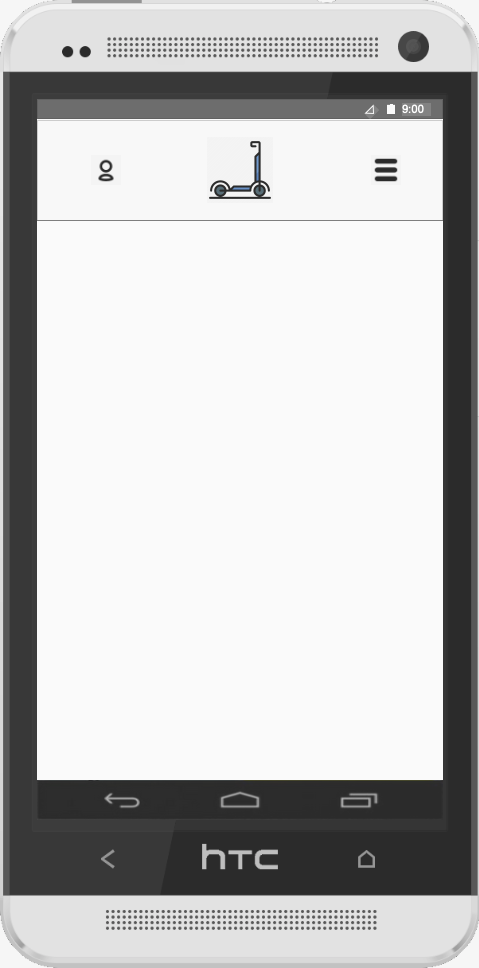
\includegraphics[scale=0.5]{images/prototypes/01-dummy.png}
  \end{center}
  \caption{Dummy}
\end{figure}

\begin{figure} [htbp]
  \begin{center}
    
\includegraphics[scale=0.5]{images/prototypes/02-start-menu.png}
  \end{center}
  \caption{Start Menu}
\end{figure}

\begin{figure} [htbp]
  \begin{center}
    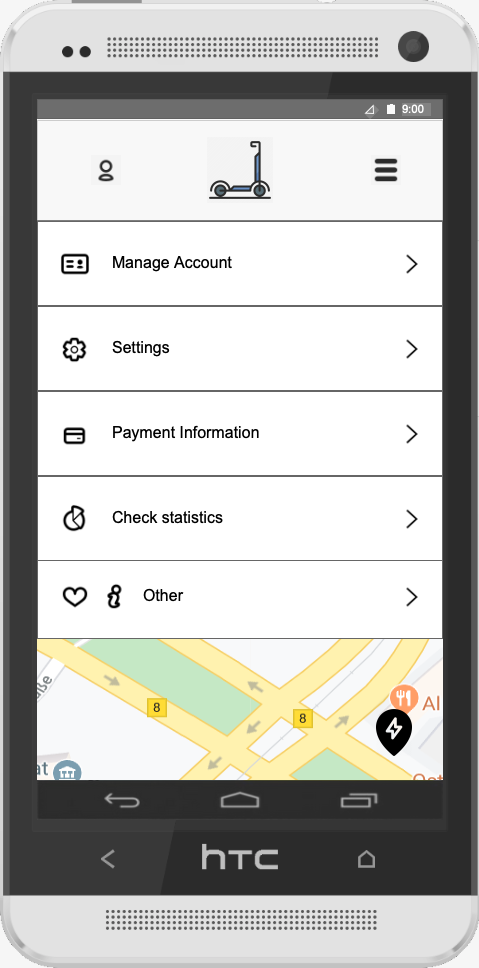
\includegraphics[scale=0.5]{images/prototypes/03-menu-dropdown.png}
  \end{center}
  \caption{Menu Dropdown}
\end{figure}

\begin{figure} [htbp]
  \begin{center}
    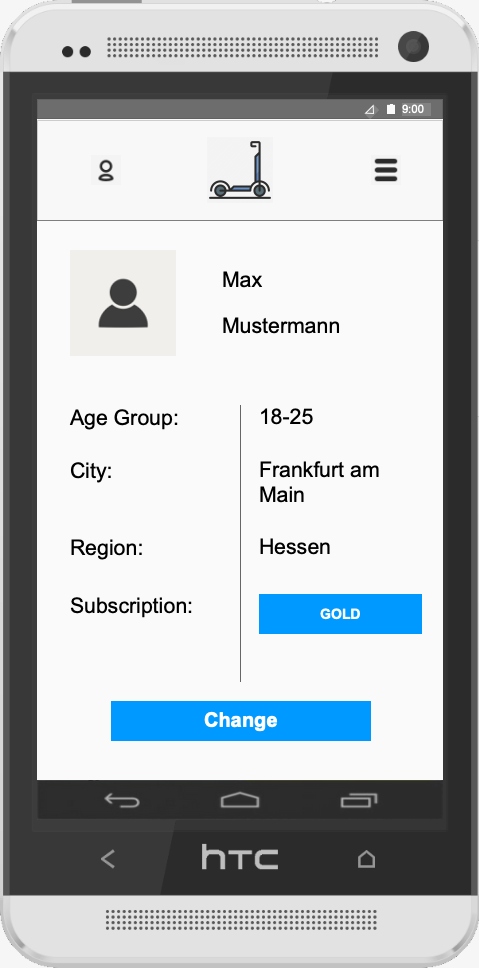
\includegraphics[scale=0.5]{images/prototypes/03-01-menu-dropdown--account-management.png}
  \end{center}
  \caption{Menu Dropdown $\rightarrow$ Account Management}
\end{figure}

\begin{figure} [htbp]
  \begin{center}
    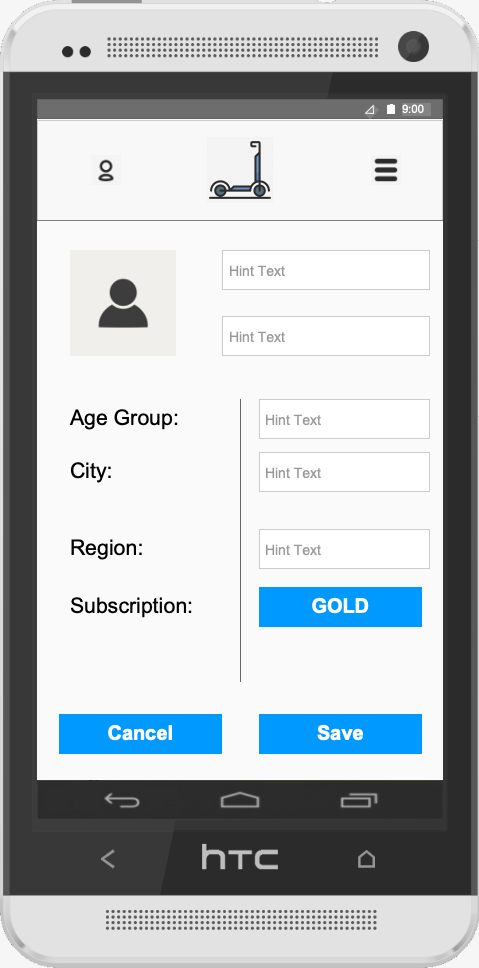
\includegraphics[scale=0.5]{images/prototypes/03-01-01-menu-dropdown--account-management--change-account-details.png}
  \end{center}
  \caption{Menu Dropdown $\rightarrow$ Account Management $\rightarrow$ Change Account Details}
\end{figure}

\begin{figure} [htbp]
  \begin{center}
    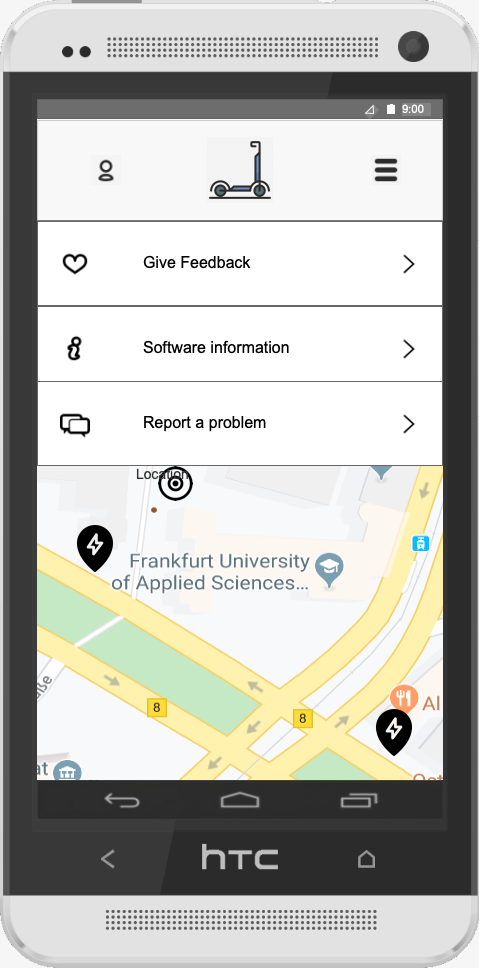
\includegraphics[scale=0.5]{images/prototypes/03-02-menu-dropdown--other.png}
  \end{center}
  \caption{Menu Dropdown $\rightarrow$ Other}
\end{figure}

\begin{figure} [htbp]
  \begin{center}
    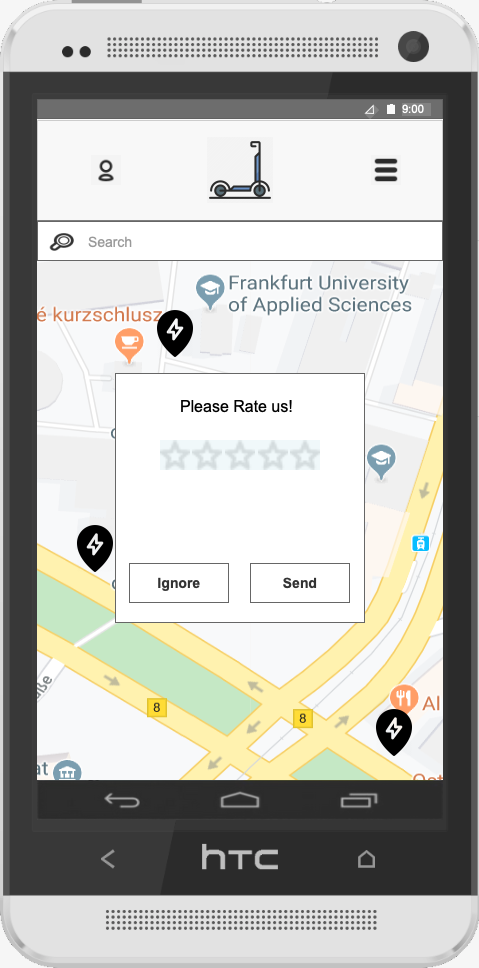
\includegraphics[scale=0.5]{images/prototypes/04-ask-for-feedback.png}
  \end{center}
  \caption{Ask for Feedback}
\end{figure}

\begin{figure} [htbp]
  \begin{center}
    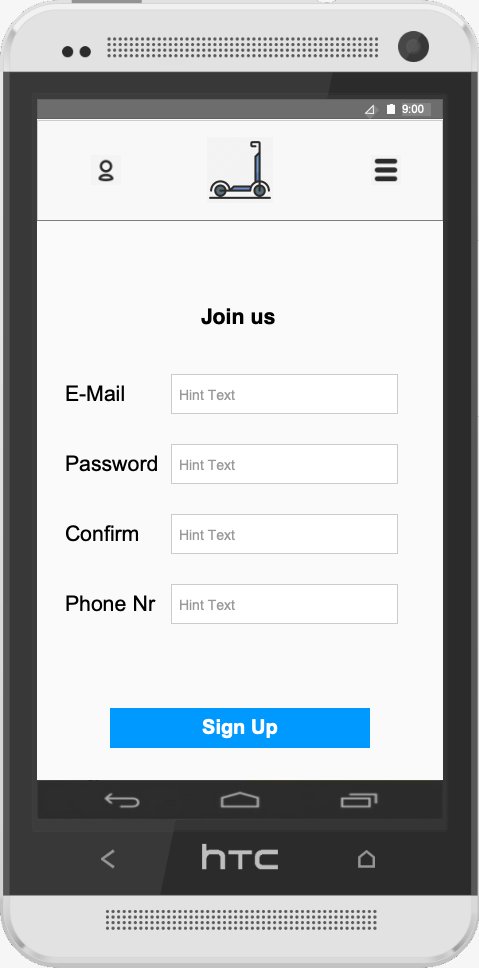
\includegraphics[scale=0.5]{images/prototypes/05-register-sign-up.png}
  \end{center}
  \caption{Register/Sign Up}
\end{figure}

\begin{figure} [htbp]
  \begin{center}
    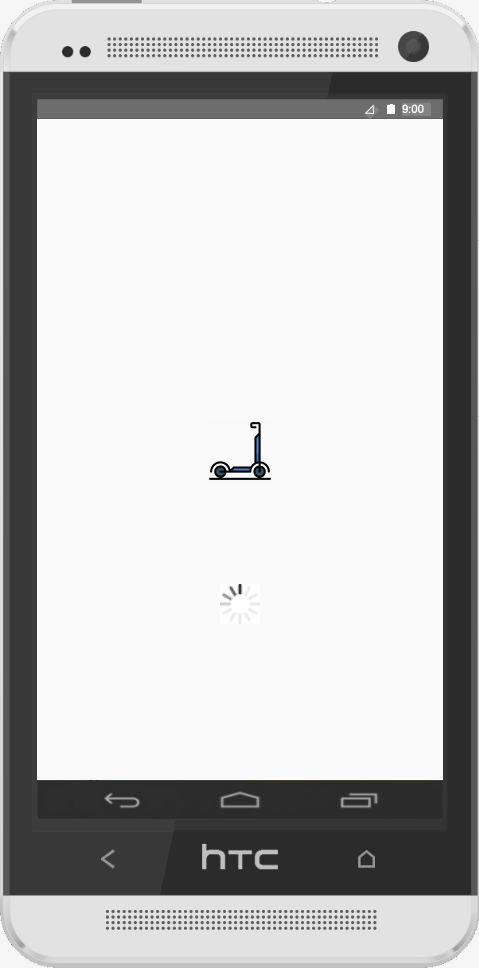
\includegraphics[scale=0.5]{images/prototypes/06-loading-screen.png}
  \end{center}
  \caption{Loading Screen}
\end{figure}

\newpage
\subsection{Meeting Protocols}


\end{document}
